\documentclass[border=15pt]{standalone}
\usepackage[utf8]{inputenc}
\usepackage[T1]{fontenc}
\usepackage{helvet}
\renewcommand{\familydefault}{\sfdefault}
\usepackage{tikz}
\usetikzlibrary{shapes,arrows.meta,positioning,calc,shadows.blur,backgrounds,decorations.pathreplacing,fit}
\usepackage{amsmath,amssymb}
\usepackage{xcolor}

% Define elegant colours
\definecolor{primary}{RGB}{41,98,255}
\definecolor{secondary}{RGB}{0,200,170}
\definecolor{accent}{RGB}{255,87,34}
\definecolor{dark}{RGB}{30,30,30}
\definecolor{light}{RGB}{250,250,252}
\definecolor{muted}{RGB}{120,120,130}

\begin{document}
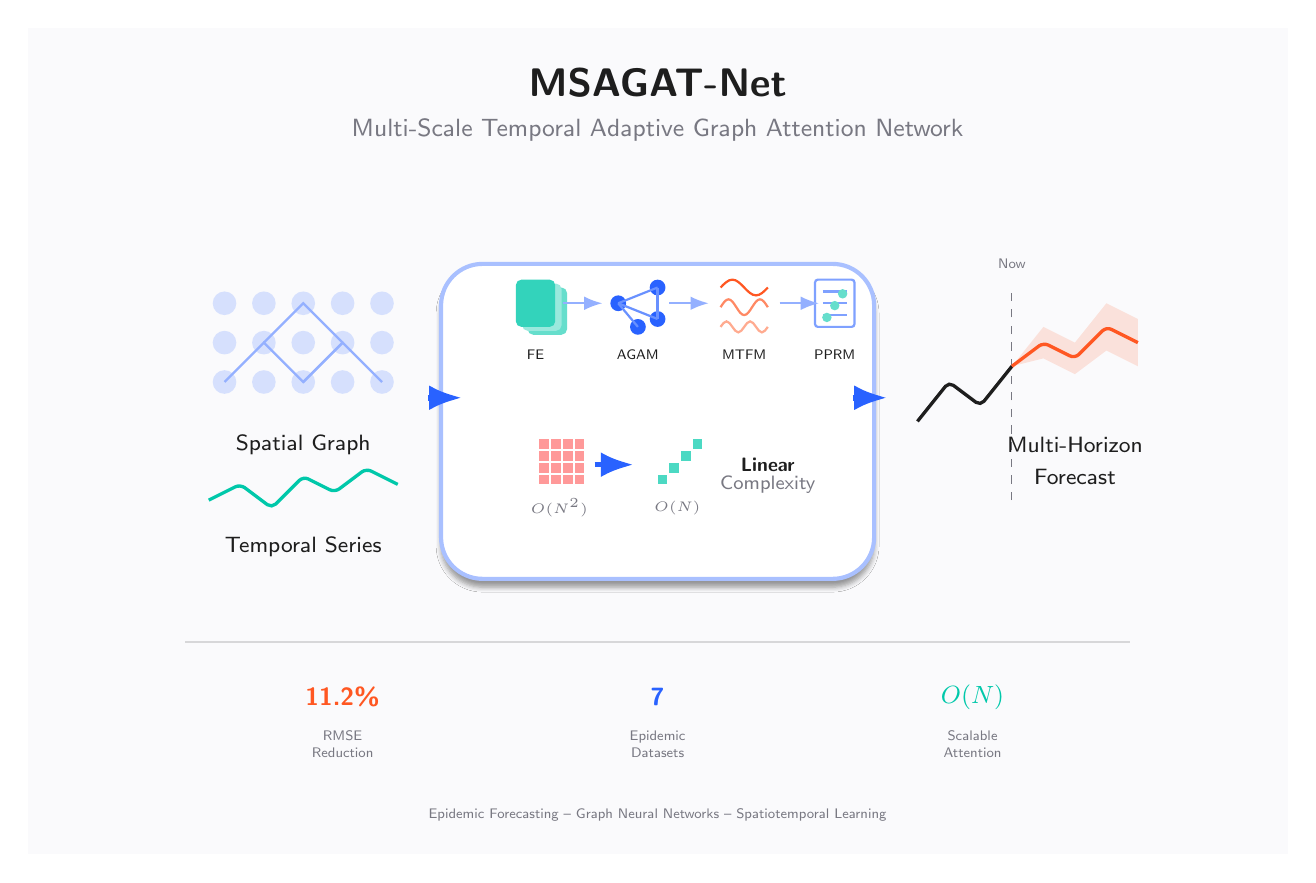
\begin{tikzpicture}[
    >=Latex
]

% ============ BACKGROUND ============
\fill[light] (-8,-5) rectangle (8,5.5);

% ============ TITLE ============
\node[font=\bfseries\Large, text=dark] at (0, 4.8) {MSAGAT-Net};
\node[font=\small, text=muted] at (0, 4.2) {Multi-Scale Temporal Adaptive Graph Attention Network};

% ============ LEFT: INPUT VISUALIZATION ============
\begin{scope}[shift={(-5.5, 1)}]
    % Stylized map/network
    \foreach \i in {0,1,2,3,4} {
        \foreach \j in {0,1,2} {
            \fill[primary!30, opacity=0.6] (\i*0.5, \j*0.5) circle (0.15);
        }
    }
    % Connections
    \draw[primary!50, thick] (0,0) -- (0.5,0.5) -- (1,0) -- (1.5,0.5);
    \draw[primary!50, thick] (0.5,0.5) -- (1,1) -- (1.5,0.5);
    \draw[primary!50, thick] (1,0) -- (1.5,0.5) -- (2,0);
    
    \node[font=\footnotesize, text=dark] at (1, -0.8) {Spatial Graph};
    
    % Time series below
    \draw[secondary, very thick, rounded corners=2pt] 
        (-0.2,-1.5) -- (0.2,-1.3) -- (0.6,-1.6) -- (1,-1.2) -- (1.4,-1.4) -- (1.8,-1.1) -- (2.2,-1.3);
    \node[font=\footnotesize, text=dark] at (1, -2.1) {Temporal Series};
\end{scope}

% ============ CENTER: MODEL (Improved) ============
\begin{scope}[shift={(0, 0.5)}]
    
    % Main container
    \node[
        rectangle,
        rounded corners=15pt,
        draw=primary!40,
        line width=1.5pt,
        fill=white,
        minimum width=5.5cm,
        minimum height=4cm,
        blur shadow={shadow blur steps=5, shadow xshift=0pt, shadow yshift=-3pt}
    ] (model) at (0,0) {};
    
    % --- Feature Extraction (layered rectangles) ---
    \begin{scope}[shift={(-1.8, 1.2)}]
        \fill[secondary!60, rounded corners=2pt] (0.15, -0.1) rectangle (0.65, 0.5);
        \fill[secondary!40, rounded corners=2pt] (0.08, -0.05) rectangle (0.58, 0.55);
        \fill[secondary!80, rounded corners=2pt] (0, 0) rectangle (0.5, 0.6);
        \node[font=\tiny, text=dark] at (0.25, -0.35) {FE};
    \end{scope}
    
    % --- AGAM (network/graph icon) ---
    \begin{scope}[shift={(-0.5, 1.2)}]
        % Nodes
        \fill[primary] (0, 0.3) circle (0.1);
        \fill[primary] (0.5, 0.5) circle (0.1);
        \fill[primary] (0.5, 0.1) circle (0.1);
        \fill[primary] (0.25, 0) circle (0.1);
        % Edges
        \draw[primary!70, thick] (0, 0.3) -- (0.5, 0.5);
        \draw[primary!70, thick] (0, 0.3) -- (0.5, 0.1);
        \draw[primary!70, thick] (0, 0.3) -- (0.25, 0);
        \draw[primary!70, thick] (0.5, 0.5) -- (0.5, 0.1);
        \node[font=\tiny, text=dark] at (0.25, -0.35) {AGAM};
    \end{scope}
    
    % --- MTFM (multi-scale waves) ---
    \begin{scope}[shift={(0.8, 1.2)}]
        \draw[accent, thick] (0, 0.5) sin (0.15, 0.6) cos (0.3, 0.5) sin (0.45, 0.4) cos (0.6, 0.5);
        \draw[accent!70, thick] (0, 0.25) sin (0.1, 0.35) cos (0.2, 0.25) sin (0.3, 0.15) cos (0.4, 0.25) sin (0.5, 0.35) cos (0.6, 0.25);
        \draw[accent!50, thick] (0, 0) sin (0.075, 0.07) cos (0.15, 0) sin (0.225, -0.07) cos (0.3, 0) sin (0.375, 0.07) cos (0.45, 0) sin (0.525, -0.07) cos (0.6, 0);
        \node[font=\tiny, text=dark] at (0.3, -0.35) {MTFM};
    \end{scope}
    
    % --- PPRM (refinement layers) ---
    \begin{scope}[shift={(2, 1.2)}]
        \draw[primary!60, thick, rounded corners=1pt] (0, 0) -- (0.5, 0) -- (0.5, 0.6) -- (0, 0.6) -- cycle;
        \draw[primary!60, thick] (0.1, 0.15) -- (0.4, 0.15);
        \draw[primary!60, thick] (0.1, 0.3) -- (0.4, 0.3);
        \draw[primary!60, thick] (0.1, 0.45) -- (0.4, 0.45);
        \fill[secondary!60] (0.35, 0.42) circle (0.06);
        \fill[secondary!60] (0.25, 0.27) circle (0.06);
        \fill[secondary!60] (0.15, 0.12) circle (0.06);
        \node[font=\tiny, text=dark] at (0.25, -0.35) {PPRM};
    \end{scope}
    
    % Flow arrows between modules
    \draw[->, primary!50, thick] (-1.2, 1.5) -- (-0.7, 1.5);
    \draw[->, primary!50, thick] (0.15, 1.5) -- (0.65, 1.5);
    \draw[->, primary!50, thick] (1.55, 1.5) -- (2.05, 1.5);
    
    % --- Complexity reduction visual ---
    \begin{scope}[shift={(0, -0.8)}]
        % O(N²) - dense matrix
        \begin{scope}[shift={(-1.5, 0)}]
            \foreach \i in {0,1,2,3} {
                \foreach \j in {0,1,2,3} {
                    \fill[red!40] (\i*0.15, \j*0.15) rectangle (\i*0.15+0.12, \j*0.15+0.12);
                }
            }
            \node[font=\tiny, text=muted] at (0.25, -0.3) {$O(N^2)$};
        \end{scope}
        
        % Arrow
        \draw[->, line width=2pt, primary] (-0.8, 0.25) -- (-0.3, 0.25);
        
        % O(N) - sparse/linear
        \begin{scope}[shift={(0, 0)}]
            \foreach \i in {0,1,2,3} {
                \fill[secondary!70] (\i*0.15, \i*0.15) rectangle (\i*0.15+0.12, \i*0.15+0.12);
            }
            \node[font=\tiny, text=muted] at (0.25, -0.3) {$O(N)$};
        \end{scope}
        
        % Label
        \node[font=\scriptsize\bfseries, text=dark] at (1.4, 0.25) {Linear};
        \node[font=\scriptsize, text=muted] at (1.4, 0) {Complexity};
    \end{scope}
    
\end{scope}

% ============ RIGHT: OUTPUT VISUALIZATION ============
\begin{scope}[shift={(5.5, 1)}]
    % Forecast visualization
    \draw[muted, dashed] (-1,-1.5) -- (-1,1.2);
    \node[font=\tiny, text=muted] at (-1, 1.5) {Now};
    
    % Historical (solid)
    \draw[dark, very thick, rounded corners=2pt] 
        (-2.2, -0.5) -- (-1.8, 0) -- (-1.4, -0.3) -- (-1, 0.2);
    
    % Forecast (gradient)
    \draw[accent, very thick, rounded corners=2pt] 
        (-1, 0.2) -- (-0.6, 0.5) -- (-0.2, 0.3) -- (0.2, 0.7) -- (0.6, 0.5);
    
    % Confidence band
    \fill[accent, opacity=0.15] 
        (-1, 0.2) -- (-0.6, 0.7) -- (-0.2, 0.5) -- (0.2, 1) -- (0.6, 0.8) --
        (0.6, 0.2) -- (0.2, 0.4) -- (-0.2, 0.1) -- (-0.6, 0.3) -- cycle;
    
    \node[font=\footnotesize, text=dark] at (-0.2, -0.8) {Multi-Horizon};
    \node[font=\footnotesize, text=dark] at (-0.2, -1.2) {Forecast};
\end{scope}

% ============ ARROWS ============
\draw[->, primary, line width=2pt, shorten >=8pt, shorten <=8pt] (-3.2, 0.8) -- (-2.2, 0.8);
\draw[->, primary, line width=2pt, shorten >=8pt, shorten <=8pt] (2.2, 0.8) -- (3.2, 0.8);

% ============ BOTTOM: KEY RESULTS ============
\node[font=\small\bfseries, text=accent] at (-4, -3) {11.2\%};
\node[font=\tiny, text=muted, align=center] at (-4, -3.6) {RMSE\\Reduction};

\node[font=\small\bfseries, text=primary] at (0, -3) {7};
\node[font=\tiny, text=muted, align=center] at (0, -3.6) {Epidemic\\Datasets};

\node[font=\small\bfseries, text=secondary] at (4, -3) {$O(N)$};
\node[font=\tiny, text=muted, align=center] at (4, -3.6) {Scalable\\Attention};

% Subtle separator line
\draw[muted!30, line width=0.5pt] (-6, -2.3) -- (6, -2.3);

% ============ FOOTER ============
\node[font=\tiny, text=muted] at (0, -4.5) {Epidemic Forecasting -- Graph Neural Networks -- Spatiotemporal Learning};

\end{tikzpicture}
\end{document}
